\documentclass[12pt]{article}
\usepackage[utf8]{inputenc}
\usepackage[UTF8]{ctex}
\usepackage{biblatex}
\usepackage{amssymb}
\usepackage{latexsym}
\usepackage{amsmath}
\usepackage{cases}
\usepackage{geometry}
\usepackage{graphicx}
\usepackage{float}
\usepackage{listings}
\usepackage{enumerate}
\usepackage{color}
\usepackage{hw1}



\usepackage{setspace}
\usepackage{multirow}
\usepackage{float}
\usepackage{fancyhdr}  % header,footer的设置
% 封面的相关命令设置
\newcommand{\hmwkTitle}{Project 1 Stamp}
\newcommand{\hmwkClass}{《现代集成电路分析方法》}
\newcommand{\hmwkCompleteTime}{\today}
\newcommand{\hmwkAuthorName}{姓名:蔡志杰 }
\newcommand{\hmwMajor}{专业:电子科学与技术}
\newcommand{\hmwNumber}{学号:22112020002}
% 用fancyhdr设置header和footer
\pagestyle{fancy}
\lhead{\hmwkClass \hmwkTitle}
\rhead{蔡志杰 \quad 22112020002}
\cfoot{\thepage}

\addbibresource{bib.bib}
\setlength{\parindent}{0em}
\bibliography{bib}
\geometry{a4paper,scale=0.8}
\linespread{1.5}
\graphicspath{{Images/}}


%%%%%%%%%%%%%
%%% COVER %%%
%%%%%%%%%%%%%
\begin{document}

\begin{titlepage}
\begin{center}
% \linespread{1.2}\huge {\bfseries Fudan University}\\[1cm]
% \linespread{1}
% \includegraphics[width=10cm]{fudan-name.pdf}\\[3cm]
% \linespread{1.9}\huge {\bfseries 可编程器件与硬件描述语言}\\
% \linespread{1.9}\LARGE {\bfseries 作业报告}\\[2.5cm]

% {\Large 姓名:名字}\\[0.3cm]
% \Large 学号:123456789\\[4cm] 
% \large 2021年11月1日



\includegraphics[scale = 0.9]{fudan.jpg}\\

\includegraphics[scale = 0.6]{fudan_logo.jpg}\\
\vspace{0.5in}
\linespread{1.9}\huge {\bfseries 现代集成电路分析方法}\\
\linespread{1.9}\LARGE {\bfseries \textbf{\hmwkTitle}}\\
\vspace{1.0in}
\large \hmwMajor{}\\
\large \hmwNumber{}\\
\large \hmwkAuthorName{}\\
% \large \date{\today} 

\end{center}
\end{titlepage}
\newpage

\begin{spacing}{1.2}
  \tableofcontents
\end{spacing}
\newpage

%%%%%%%%%%%%%%%%%
%%% MAIN TEXT %%%
%%%%%%%%%%%%%%%%%

\section{设计指标}
\qquad 设计一个程序根据输入的线性电路网表生成相应的MNA方程:
\begin{gather*}
C \dot{X}+G X=B U \\
Y=L^T X 
\end{gather*}
\quad 其中$X$为包含所有节点(普通节点(电压变量)和辅助节点(电流变量))的列向量,$\dot{X}$为对应变量的导数,$Y$为所有输出节点组成的列向量,$U$为所有独立源组成的列向量,$C、G、B、L^T$则为系数矩阵。\par
\subsection{输入文件}
\qquad 输入的线性电路为SPICE格式的网表文件 \par
\qquad (1)能至少处理6种元件: R,L,C,K(互感),V(独立电压源),I(独立电流源)。 \par
\qquad (2)应能处理子电路,不用考虑全局节点(0节点除外)。 \par
\qquad (3)用一下语句生成输出变量Y: \par
\qquad \qquad .PROBE V(node1) V(node2)... \par
\qquad 其中node1、node2为要观察的节点的名称。(SPICE不区分大小写)

\subsection{输出结果}
\qquad 输出为一个或多个文件,应包含以下内容:\par
\qquad (1)各矩阵或向量的大小。\par
\qquad (2)X中各未知量的具体代表内容。U中各源的名称。Y各量的具体代表内容。\par
\qquad (3)$C,G,B,L^T$应以二进制格式存储,以保证精度。\par
\qquad 此外需要提供一个MAT函数能支持读取输出的文件,将其对应的矩阵存储到MATLAB内存中。\par

\subsection{进一步的工作}
\qquad (1)程序运行过程和最终结果采用稀疏矩阵存储。\par
\qquad (2)生成分块结构的MNA方程.\par
\qquad (3)支持更多的元件:E(电压控制的电压源),G(电压控制的电流源),H(电流控制的电压源),F(电流控制的电流源)。\par

\section{算法原理} \label{sec:2}

\qquad 电路分析需要根据电路中的元件特性及其连接关系得到一系列的电路方程,进而求解得到电路的特性。电路方程都是基于基尔霍夫电压定律(KVL)、基尔霍夫电流定律(KCL)和电路元件自身的电流电压方程所构建的。传统的节点电压法和回路电流法不适用于计算机求解,MNA(Modified Node Analysis)改良节点分析则是构建了MNA方程,再通过分析各个元件对MNA方程的贡献来逐步构建起MNA方程。\par

\begin{gather*}
  C \dot{X}+G X=B U
  \end{gather*}
\begin{equation*}
  \left[\begin{array}{ll}
  C & 0 \\
  0 & L
  \end{array}\right]\left[\begin{array}{l}
  \dot{V} \\
  \dot{I}
  \end{array}\right]+\left[\begin{array}{cc}
  G & E \\
  -E^T & 0
  \end{array}\right]\left[\begin{array}{l}
  V \\
  I
  \end{array}\right]=B U
\end{equation*}
\qquad 上面两个方程展示了原始MNA方程和分块MNA方程,Stamp算法的处理思路则是按顺序单独考虑每一个电路元件对MNA方程中矩阵的影响,这样便于计算机程序进行处理。\par
\qquad 接下来分析一下在Stamp方法中各种元件对各个矩阵的影响。\par

\subsection{电阻$R$} \label{subsec:2.1}
\begin{equation*}
  i_R(t)=\frac{1}{R}\left(V_i(t)-V_j(t)\right)
\end{equation*}
\begin{table}[H]
  \centering
  \renewcommand\arraystretch{0.5}
  \begin{tabular}{ccccc}
    & $ \qquad \qquad i \qquad \quad  j$ & & & \\                            \\
  $\left[C_R\right]=0$ & 
  $\left[G_R\right]= \left[\begin{array}{cc} 1 / R & -1 / R \\ -1 / R & 1 / R \end{array}\right]$  & 
  $\begin{array}{c} i \\ j \end{array}$ & 
  $\left[B_R\right]=0$ & 
  $\left[X_R\right]=\left[ V_i \ V_j \right]^T$ \\
  \end{tabular}
\end{table}
\qquad SPICE语法: Rname Pnode Nnode Value\par
\qquad 其中$i$和$j$分别对应着电阻正负节点(SPICE语法:中的Pnode和Nnode)在MNA矩阵中对应的序号(后文中$i$和$j$的含义也相同)。电阻只会影响$G$矩阵。\par
\qquad 若需要为阻引入电流变量(当流经电阻的电流作用于受控源时),stamp操作如下式所示,会改变$G$矩阵。\par
\begin{table}[H]
  \centering
  \renewcommand\arraystretch{0.5}
  \begin{tabular}{cccccc}
   & & $ \qquad \quad i \quad j \quad k$ & & & \\                            \\
  $\left[C_C\right]=0$  & 
  $\begin{array}{c} i \\ j \\ k \end{array}$& 
  $\left[G_C\right]=\left[\begin{array}{ccc} 0 & 0 & 0\\ 0 & 0 & 0\\ 1 & -1 & -R \end{array}\right]$  & 
  $\begin{array}{c} i \\ j \\ k \end{array}$ & 
  $\left[B_C\right]=0$ & 
  $\begin{array}{c} \qquad i \quad j \quad k \\ \left[X_C\right]=\left[ V_i \ V_j \ I_C \right]^T\end{array}$ \\
  \end{tabular}
\end{table}

\subsection{电容$C$} \label{subsec:2.2}
\begin{equation*}
  i_C(t)=C\left(\dot{V_i}(t)-\dot{V_j}(t)\right)
\end{equation*}
\begin{table}[H]
  \centering
  \renewcommand\arraystretch{0.5}
  \begin{tabular}{ccccc}
  $ \qquad \qquad i \qquad \quad  j$ &  & & & \\                            \\
  $\left[C_C\right]=  \left[\begin{array}{cc} C & -C \\ -C & C \end{array}\right]$  & 
  $\begin{array}{c} i \\ j \end{array}$& 
  $\left[G_C\right]=0$ & 
  $\left[B_C\right]=0$ & 
  $\left[X_C\right]=\left[ V_i \ V_j \right]^T$ \\
  \end{tabular}
\end{table}
\qquad SPICE语法: Cname Pnode Nnode Value <IC>\par
\qquad 电容只对$C$矩阵有贡献。\par
\qquad 若需要为电容引入电流变量(当流经电容的电流作用于受控源时),stamp操作如下式所示,会改变$C$和$G$矩阵。\par
\begin{table}[H]
  \centering
  \renewcommand\arraystretch{0.5}
  \begin{tabular}{cccccc}
  $ \qquad \quad i \quad j \quad k$ & & $ \qquad \quad i \quad j \quad k$ & & & \\                            \\
  $\left[C_C\right]=\left[\begin{array}{ccc} 0 & 0 & 0\\ 0 & 0 & 0\\ 1 & -1 & 0 \end{array}\right]$  & 
  $\begin{array}{c} i \\ j \\ k \end{array}$& 
  $\left[G_C\right]=\left[\begin{array}{ccc} 0 & 0 & 0\\ 0 & 0 & 0\\ 0 & 0 & -1 / C \end{array}\right]$  & 
  $\begin{array}{c} i \\ j \\ k \end{array}$ & 
  $\left[B_C\right]=0$ & 
  $\begin{array}{c} \qquad i \quad j \quad k \\ \left[X_C\right]=\left[ V_i \ V_j \ I_C \right]^T\end{array}$ \\
  \end{tabular}
\end{table}

\subsection{电感$L$}
\begin{equation*}
  L\dot{i_L}(t)=C\left(\dot{V_i}(t)-\dot{V_j}(t)\right)
\end{equation*}
\begin{table}[H]
  \centering
  \renewcommand\arraystretch{0.5}
  \begin{tabular}{cccccc}
  $ \qquad \quad i \quad j \quad k$ & & $ \qquad \quad i \quad j \quad k$ & & & \\                            \\
  $\left[C_L\right]=\left[\begin{array}{ccc} 0 & 0 & 0\\ 0 & 0 & 0\\ 0 & 0 & L \end{array}\right]$  & 
  $\begin{array}{c} i \\ j \\ k \end{array}$& 
  $\left[G_L\right]=\left[\begin{array}{ccc} 0 & 0 & 1\\ 0 & 0 & -1\\ -1 & 1 & 0 \end{array}\right]$  & 
  $\begin{array}{c} i \\ j \\ k \end{array}$ & 
  $\left[B_L\right]=0$ & 
  $\begin{array}{c} \qquad i \quad j \quad k \\ \left[X_L\right]=\left[ V_i \ V_j \ I_L \right]^T\end{array}$ \\
  \end{tabular}
\end{table}
\qquad SPICE语法: Iname Pnode Nnode Value <IC>\par
\qquad 为了描述电感的电流需要引入一个额外的变量,在MNA中对应一个辅助节点(aux\_node),$k$ 为电感引入的辅助节点的序号。电感对$C$和$G$矩阵均有贡献。\par

\subsection{互感$K$} \label{subsec:2.4}
\begin{equation*}
  \left\{\begin{array}{l}
  v_1(t)=L_1 \frac{d i_1(t)}{d t}+M_{12} \frac{d i_2(t)}{d t} \\
  v_2(t)=M_{12} \frac{d i_1(t)}{d t}+L_2 \frac{d i_2(t)}{d t}
  \end{array}\right.
\end{equation*}
\begin{equation*}
  {\rm Coupling \quad coefficient} \qquad  k=\frac{M}{\sqrt{L_1 L_2}} \quad\left(M_{12}=M_{21}=M\right)
\end{equation*}
\begin{table}[H]
  \centering
  \renewcommand\arraystretch{0.5}
  \begin{tabular}{ccccc}
  $ \qquad \qquad i \qquad \quad  j$ &  & & & \\                            \\
  $\left[C_K\right]=  \left[\begin{array}{cc} 0 & -M \\ -M & 0 \end{array}\right]$  & 
  $\begin{array}{c} i \\ j \end{array}$& 
  $\left[G_K\right]=0$ & 
  $\left[B_K\right]=0$ & 
  $\begin{array}{c} \qquad i \quad j \\ \left[X_K\right]=\left[ I_{L1} \ I_{L2} \right]^T\end{array}$ \\
  \end{tabular}
\end{table}
\qquad SPICE语法: Kname Inductor1 Inductor2 Value\_of\_k <IC>\par
\qquad 这里的$i$和$j$分别指电感$L1$和$L2$对应的辅助节点的序号。互感只对$C$矩阵有贡献。\par

\subsection{独立电流源$I_{src}$}
\begin{table}[H]
  \centering
  \renewcommand\arraystretch{0.5}
  \begin{tabular}{cccc}
  $\left[C_{CS}\right]=0$ & 
  $\left[G_{CS}\right]=0$ & 
  $\left[B_{CS}\right]=\left[ -I_{CS} \ I_{CS} \right]^T$ & 
  $\left[X_{CS}\right]=\left[ V_{i} \ V_{j} \right]^T$ \\
  \end{tabular}
\end{table}
\qquad SPICE语法: Iname Pnode Nnode <Type> Value\par
\qquad  独立电流源只对$B$矩阵有贡献,在stamp的过程中需要给每个电流源在矩阵$U$中确定输入源的序号,独立电流源对$B$矩阵贡献的位置将取决于电源的序号以及电源正负节点对应的序号。SPICE语法中的Type对应着独立电流源的种类(如交流或直流),实际中独立电流源和电压源的种类更多,语法也更加复杂,这里默认解析上面这种语法,若没提供种类则默认直流,否则种类后只跟一个数值。(假设电流源的电流的方向为从正节点流到负节点,即对正节点为流出,对负节点为流入)\par

\subsection{独立电压源$V_{src}$}
\begin{equation*}
  V_{src}=\left(V_i - V_j\right)
\end{equation*}
\begin{table}[H]
  \centering\renewcommand\arraystretch{0.5}
  \begin{tabular}{ccccc}
   & $ \qquad \quad i \quad j \quad k$ & & & \\                            \\
  $\left[C_{VS}\right]=0$ & 
  $\left[G_{VS}\right]=\left[\begin{array}{ccc} 0 & 0 & 1\\ 0 & 0 & -1\\ -1 & 1 & 0 \end{array}\right]$  & 
  $\begin{array}{c} i \\ j \\ k \end{array}$ &
  $\begin{array}{c} \qquad i \quad j \quad k \\ \left[B_{VS}\right]=\left[ 0 \ 0 \ E_{VS} \right]^T \end{array}$ & 
  $\begin{array}{c} \qquad i \quad j \quad k \\ \left[X_{VS}\right]=\left[ V_{i} \ V_{j} \ I_{VS} \right]^T \end{array}$ \\
  \end{tabular}
\end{table}
\qquad SPICE语法: Vname Pnode Nnode <Type> Value\par
\qquad 为了描述独立电压源的电流需要引入一个辅助节点,$k$则对应了这个辅助节点的序号。独立电压源对$G$和$B$矩阵都有贡献,同样为了确定独立电压源对矩阵$B$的贡献位置需要获得电源在矩阵$U$中的序号。(假设电压源的电流变量的方向为从负节点流到正节点,即对正节点为流入,对负节点为流出,之后的受控电压源的电流方向也按照这样定义)\par

\subsection{电流控制的电流源$F(CCCS)$}
\begin{equation*}
  I_{CCCS}=F·I_{Ctrl}
\end{equation*}
\begin{table}[H]
  \centering\renewcommand\arraystretch{0.5}
  \begin{tabular}{ccccc}
   & $ \qquad \quad i \quad j \quad k$ & & & \\                            \\
  $\left[C_{F}\right]=0$ & 
  $\left[G_{F}\right]=\left[\begin{array}{ccc} 0 & 0 & F\\ 0 & 0 & -F \\ 0 & 0 & 0\end{array}\right]$  & 
  $\begin{array}{c} i \\ j \\ k\end{array}$ &
  $\left[B_{F}\right]=0$ & 
  $\begin{array}{c} \qquad i \quad j \quad k\\ \left[X_{F}\right]=\left[ V_i\ V_j\ I_{Ctrl}\right]^T \end{array}$ \\
  \end{tabular}
\end{table}
\qquad SPICE语法: Fname Pnode Nnode Vcontrol Value\par
\qquad 在SPICE语法中的Vcontrol通常是一个元件的名称,以流过这个元件的电流作为控制电流,当这个元件本身已经引入了相应的电流变量和辅助节点时(如电感L和独立电流源V),$k$则对应了这个辅助节点的序号,但若控制元件没本身没有辅助节点(如电阻R和电容C)则需要为其引入相应的电流变量和辅助节点(这里增加一个辅助节点即电流变量是为了运算的方便,实际上对于R/C也可以直接用现有的节点来表示电流,但是加入新的节点可以使得在处理的阶段更加有条理,为电阻和电容增加辅助节点的方法可以参见章节\ref{subsec:2.1}和章节\ref{subsec:2.2}),$k$同样为这个辅助节点的序号。电流控制的电流源对$G$矩阵有贡献。\par

\subsection{电流控制的电压源$H(CCVS)$}
\begin{equation*}
  V_{CCVS}=V_{CCVSP} - V_{CCVSN}=H·I_{Ctrl}
\end{equation*}
\begin{table}[H]
  \centering\renewcommand\arraystretch{0.5}
  \begin{tabular}{ccccc}
   & $ \qquad \quad i \quad j \quad k \quad l$ & & & \\                            \\
  $\left[C_{H}\right]=0$ & 
  $\left[G_{H}\right]=\left[\begin{array}{cccc} 0 & 0 & -1 & 0 \\ 0 & 0 & 1 & 0 \\ 1 & -1 & 0 & -H \\ 0 & 0 & 0 & 0\end{array}\right]$  & 
  $\begin{array}{c} i \\ j \\ k \\ l\end{array}$ &
  $\left[B_{H}\right]=0$ & 
  $\begin{array}{c} \qquad \quad i \quad j \quad k \quad l\\ \left[X_{H}\right]=\left[ V_{i}\ V_{j}\ I_{CCVS}\ I_{Ctrl}\right]^T \end{array}$ \\
  \end{tabular}
\end{table}
\qquad SPICE语法: Hname Pnode Nnode Vcontrol Value\par
\qquad 为了描述电流控制电压源的电流,需要为电流控制电压源引入相应的电流变量和辅助节点,节点序号为$k$。同样控制电流也有相应的辅助节点,其对应序号为$l$(当控制元件没有电流变量(辅助节点时)同样也需要为其增加一个辅助变量)。电流控制的电压源对$G$矩阵有贡献。\par

\subsection{电压控制的电流源$G(VCCS)$}
\begin{equation*}
  I_{VCCS}=F·V_{Ctrl}=G·\left(V_{CtrlP} - V_{CtrlN}\right)
\end{equation*}
\begin{table}[H]
  \centering\renewcommand\arraystretch{0.5}
  \begin{tabular}{ccccc}
   & $ \qquad \quad i \quad j \quad k \quad l$ & & & \\                            \\
  $\left[C_{G}\right]=0$ & 
  $\left[G_{G}\right]=\left[\begin{array}{cccc} 0 & 0 & G & -G \\ 0 & 0 & -G & G \\ 0 & 0 & 0 & 0 \\ 0 & 0 & 0 & 0\end{array}\right]$  & 
  $\begin{array}{c} i \\ j \\ k \\ l\end{array}$ &
  $\left[B_{G}\right]=0$ & 
  $\begin{array}{c} \qquad \quad i \quad j \quad k \quad l\\ \left[X_{G}\right]=\left[ V_{i}\ V_{j}\ V_{CtrlP}\ V_{CtrlN}\right]^T \end{array}$ \\
  \end{tabular}
\end{table}
\qquad SPICE语法: Gname Pnode Nnode PControlNode NControlnode Value\par
\qquad 式中$k$和$l$分别对于控制的正负节点即PControlNode NControlnode。电流控制的电压源对$G$矩阵有贡献。\par

\subsection{电压控制的电压源$E(VCVS)$}
\begin{equation*}
  V_{VCCS}=V_{VCCSP} - V_{VCVSN}=E·V_{Ctrl}=E·\left(V_{CtrlP} - V_{CtrlN}\right)
\end{equation*}
\begin{table}[H]
  \centering\renewcommand\arraystretch{0.5}
  \begin{tabular}{ccccc}
   & $ \qquad \quad i \quad j \quad k \quad l \quad m$ & & & \\                            \\
  $\left[C_{E}\right]=0$ & 
  $\left[G_{E}\right]=\left[\begin{array}{ccccc} 0 & 0 & 0 & 0 & -1 \\ 0 & 0 & 0 & 0 & 1 \\ 0 & 0 & 0 & 0 & 0 \\ 0 & 0 & 0 & 0 & 0\\ 1 & -1 & -E & E & 0\end{array}\right]$  & 
  $\begin{array}{c} i \\ j \\ k \\ l \\m\end{array}$ &
  $\left[B_{E}\right]=0$ & 
  $\begin{array}{c} \qquad \quad i \quad j \quad k \quad l \quad m\\ \left[X_{E}\right]=\left[ V_{i}\ V_{j}\ V_{CtrlP}\ V_{CtrlN}\ I_{VCVS}\right]^T \end{array}$ \\
  \end{tabular}
\end{table}
\qquad SPICE语法: Ename Pnode Nnode PControlNode NControlnode Value\par
\qquad 式中$k$和$l$分别对于控制的正负节点即PControlNode NControlnode,为了表示电压控制电压源的电流变量,引入新的辅助节点,$m$为其序号。电流控制的电压源对$G$矩阵有贡献。\par

\section{算法实现}

\qquad 为了实现从SPICE网表生成MNA矩阵的过程,整个算法可以分为三大步骤:\par
\begin{itemize}
  \item 对输入的网表文件进行解析,得到相应的器件信息(如器件的连接关系、器件的值等),同时能够递归地解析嵌套的子电路。解析完网表文件后进行预处理(增加相应的电流变量和辅助节点,确定独立电流、电压源的序号)
  \item 对每个器件进行stamp操作,完成电路的MNA方程。
  \item 将得到的MNA矩阵输出为二进制格式的数据。
\end{itemize}
\begin{gather*}
C \dot{X}+G X=B U \\
Y=L^T X 
\end{gather*}
\quad 为了提高输出文件的可读性,$C、G、B、L^T$存储的为浮点数,$X、Y、U$存储的为字符串,对应了相应的变量名。同时增加了一个和列向量$U$大小相同的列向量$I$存储U向量中输入对应的数值(如独立电压/流源的电压/流)。\par
\qquad 接下来将分别对各个步骤以及一些底层的实现进行介绍。\par

% \subsection{算法流程及结构}

\subsection{解析SPICE网表}
\qquad 基于原有的parser框架进行修改和完善,增加了解析子电路和四种受控源的部分。 \par

\subsubsection{解析电路元件和输出节点}
\qquad 对于电路元件,相应的SPICE语法按照章节\ref{sec:2}中介绍的进行解析。为了方便后续分块矩阵的实现,将普通节点(电压节点)和辅助节点(电流变量)分开存储。在解析过程中就先对普通节点进行编号,当所有元件都已经解析完,所有辅助节点都以及生成好后,再对辅助节点按照元件的类别的顺序生成序号,这样能保证辅助节点的序号都在普通节点之后。\par
\qquad 对于输出节点的解析,SPICE的语法是\quad .PROBE \quad V(node1) \quad V(node2) ...。其中node1、node2为要观察的节点名称(通常为普通节点),只要解析到所有要观察的节点就能得到输出矩阵Y的变量。\par

\subsubsection{解析子电路}
\qquad 在SPICE中子电路的定义语法为:\par
\qquad .SUBCKT \quad SUBNAME \quad N1 \quad N2 \quad N3 \quad ... \par
\qquad Element \quad statements\par
\qquad .\par
\qquad .\par
\qquad .ENDS \quad SUBNAME\par
\qquad 子电路的调用方法为:\par
\qquad Xname \quad N1 \quad N2 \quad N3 \quad ... \quad SUBNAME\par
\qquad 其中SUBNAME为子电路的名称,N1、N2、N3...为子电路的接口, Xname则为实例化子电路的名称。由于子电路的定义可能在实例化之后,而且子电路还可能出现嵌套调用的情况(即子电路中包含别的子电路的实例),因此为解析子电路单独构建了一个解析函数打包在Subckt类下。该类只有一个实例化函数instantiate,每当解析到SPICE中的实例化语句时会进行调用(以X开头的语句)。实例化函数的运行流程是先根据实例化语句获取实例化子电路的名称、接口节点名称以及子电路名称,然后根据子电路名称从网表文件中查找子电路的定义语句,然后解析子电路对应语句中的电路元件。为了避免重名,子电路中电路元件的名称后面会加上\#和子电路实例名。同时对于子电路中的节点,如果为子电路的端口节点(即定义在.SUBCKT SUBNAME ...这一行的节点名)则将其名字对应到实例化子电路的接口节点名称中,同时0节点作为全局节点若识别到也会直接映射到序号0,此外的节点为子电路的内部节点,需要添加新的节点,并为其分配序号,同时节点的命名也是节点原先名字加上\#和子电路实例名。这里对子电路的操作会影响到一些电路数据(如新增的节点,新增的元件),为了函数调用时方便,将算法操作过程中所需的一些变量都打包到一个db类中(包含MNA的各个矩阵变量、元件信息、节点信息等),调用子电路解析函数时只需要将db类的引用作为参数传递进去。同时在子电路解析过程中如果再次遇到子电路实例化语句则会递归调用instantiate函数,继续解析,以实现解析嵌套子电路的功能。\par

\subsubsection{元件预处理}
\qquad 在解析网表文件的过程中,为了实现分块矩阵(节点矩阵$X$的有序性)暂时没有直接为辅助节点确定序号,同时还有一些元件也需要后续处理一下(增加额外的辅助节点,绑定相关电感等)这些操作都将在元件预处理中进行。\par
\qquad 由于预处理中需要遍历某一类型的元件,在解析过程中为各种元件独立设置了一个map来存储其对应的元件索引(一个从字符串映射到整数集合的map,字符串为元件的类型如"R"、"C",整数集合则为这一类型的元件索引),接下来遍历所有的电感、独立电压源、电压控制的电压源和电流控制的电压源,为其绑定额外节点的序号。然后遍历独立电源为其绑定电源的序号。接着遍历所有互感,为其绑定两个相应的电感、辅助节点和计算互感值。最后遍历电流控制的电压源和电流控制的电流源,确定其控制源是否存在电流变量,存在则之间绑定控制源的辅助节点序号,不存在则要为其增加新的辅助节点,然后再绑定辅助节点序号。\par
\subsection{电路元件实现}

\qquad 为了简化元件的表示,将元件共有的属性提取成一个抽象基类Device(具有元件名称\_name、正负节点序号\_p/nnode、元件的值\_value、辅助节点序号\_aux\_node和名字\_aux\_name、是否具有辅助节点的标志位\_exist\_aux\_node(同时包含相应成员变量的设置set和访问get接口),以及stamp函数(纯虚函数))。为了方便受控源的实现,为其也建立了一个基类CtrlSrc,以Device为基类,额外增加了控制元件的正负节点\_ctrl\_p/nnode,以及控制元件的名称\_ctrl\_name,同样也包含设置和访问相应成员变量的接口。\par
\qquad 为了表示每一个元件,为每一种类别的元件都创建一个C++类,电阻Resistor、电容Capacity、电感Inductor、互感Mutual、独立电流源Isrc和独立电压源Vsrc则是直接继承与Device基类,其中互感需要额外增加成员变量:互感的值\_mut\_value(可通过章节\ref{subsec:2.4}中的公式计算得到)、两个电感的名字\_ind1/2和两个电感对于的辅助节点的序号\_aux\_node\_ind1/2。对于独立电流源和电压源,则需要增加表示电源类型的成员变量\_type和电源对于的序号\_src\_idx(在$U$矩阵中的序号)。\par
\qquad 电压控制的电压源Vcvs、电压控制的电流源Vccs、电流控制的电压源Ccvs和电流控制的电流源Cccs则继承与CtrlSrc基类。其中电流控制的电压源和电流源需要增加以下的成员变量:控制元件的名字\_ctrl\_name、控制元件的辅助节点序号\_ctrl\_aux\_node、控制节点的值\_ctrl\_value(电阻就为阻值,电容就为容值,用于为之前没有辅助节点的电阻和电容创造辅助节点所需的方程,体现在MNA系数矩阵中,对矩阵的修改方法详见章节\ref{subsec:2.1}和章节\ref{subsec:2.2})以及控制元件是否存在辅助节点的标志位\_exist\_ctrl\_aux(不存在则需在stamp操作中为辅助节点进行相应的操作,创造辅助节点的步骤会在解析后的元件预处理中进行)。\par
\qquad 各个元件的stamp操作则按照章节\ref{sec:2}中描述的进行。\par

\subsection{矩阵实现}
\qquad 由于MNA的系数矩阵具有稀疏的特点,因此可以实现稀疏矩阵更能节省空间,所有对于MNA的稀疏矩阵需要实现的功能主要有基于底层稀疏矩阵的数据结构,实现对矩阵某一元素访问get并加减add的功能,同时为了更方便地获得矩阵的某一部分(打印出相应的分块矩阵)还实现了根据根据子矩阵的其实坐标和子矩阵的大小,从矩阵中通过切片获得子矩阵的接口getSubMatrix。\par 
\qquad 为了输出的方便,为矩阵提供了几个输出的接口output(普通输出,会按照矩阵大小,将完整的矩阵打印出来,没有元素的地方会用0填补),sparse\_output(输出矩阵的稀疏新式即每行只包括对应元素的(row,\ col)\ value)和binary\_output(将矩阵按照二进制形式打印出来,开头打印三个数字,分别对应矩阵的总行数、总列数以及非零元素个数,后续每行包括每个非零元素的行、列和值这三个数,打印出的文件存储于.dat文件中,方便matlab函数读取)。\par
\qquad 此外每个矩阵还有一些成员变量:矩阵的大小(总行列数)、矩阵的名字(便于打印的时候验证)。\par
\subsubsection{稀疏存储}
\qquad 虽然原始代码中建议用十字链表来实现矩阵的稀疏存储,但是考虑到链表这一结构访问的元素的速度还不够快,因此本算法采用c++标准库中的map进行实现,矩阵底层数据的类型为std::map<int, std::map<int,T>>其中T为矩阵的模板变量,可以存储不同类型的矩阵,由于map底层的实现是红黑树,在数据存储上稀疏程度与链表接近,同时红黑树的查找时间复杂度为O(log(N))(十字链表是O(N),二维数组是O(1)),其中N为该行/列的非0元素数量,算是在内存和运行时间上取得了一个较好的权衡。\par
\subsubsection{分块矩阵}
\qquad 由于前面解析和预处理过程以及将节点按照类别进行排序(电压节点在前,辅助节点在后),同时辅助节点也有按照类型进行排序,因此直接按照完整矩阵进行切割即可得到相应的分块矩阵。因此只要实现子矩阵获取功能即可得到分块矩阵。(经分析当电流控制的电压源的控制源有辅助节点时,$G$矩阵右下角的子矩阵都不为全零矩阵。)\par
\begin{equation*}
  \left[\begin{array}{ll}
  C & 0 \\
  0 & L
  \end{array}\right]\left[\begin{array}{l}
  \dot{V} \\
  \dot{I}
  \end{array}\right]+\left[\begin{array}{cc}
  G & E \\
  -E^T & 0
  \end{array}\right]\left[\begin{array}{l}
  V \\
  I
  \end{array}\right]=B U
\end{equation*}

\subsubsection{Matlab读取矩阵}
\qquad 对输出的二进制文件,编写了matlab函数read\_matrix来读取C++程序输出的二进制文件,读取的时候先用一个3xn的矩阵来存储数据(其中n为矩阵非0元素的个数,每一列为非零元素的行坐标、列坐标和值),然后再用matlab的sparse函数将其转换成稀疏矩阵。\par

\section{编译运行与结果}

\qquad 为了使得本次项目的结构更加清晰,将原始的源文件加头文件的格式换成了hpp的文件格式,每一个类都对应一个hpp文件,同时编写了CMakeLists.txt来方便文件的编译。\par
\subsubsection{编译运行}
\qquad 编译方法:\par
\qquad cd ./project/src\par
\qquad mkdir build\par
\qquad cd ./build\par
\qquad cmake ..\par
\qquad make\par
\qquad 运行方法:\par
\qquad ./MNA infile.sp \par
\qquad 其中infile.sp为输入的SPICE网表,将会在当前目录自动输出五份文件,分别为infile\_binary.dat(输出的二进制矩阵数据),infile\_full.txt(输出的完整矩阵,用于观察),infile\_sparse.txt(输出的稀疏矩阵,用于观察),infile\_sub\_matrix.txt(输出的分块矩阵) infile\_zero.txt(输出分块矩阵中对应全零的矩阵用于验证是否满足全0的要求)。\par
\qquad 编译环境为Linux系统,gcc版本为9.4.0。\par

\subsubsection{运行结果}

\qquad 运行结果如下图所示,由于Bus和Tree两个例子的规模太大没办法展示完全,故以Test和RLC两个例子为例。(为了方便展示将输出文件中的各个矩阵截图后拼接了一下,原始数据可以参见/output/RLC\_s3\_full.txt和/output/Test\_0\_full.txt)。对RLC和Test网表进行了手动验算,发现结果与矩阵输出一致。\par
\qquad \par
\begin{figure}[H]
  \centering
  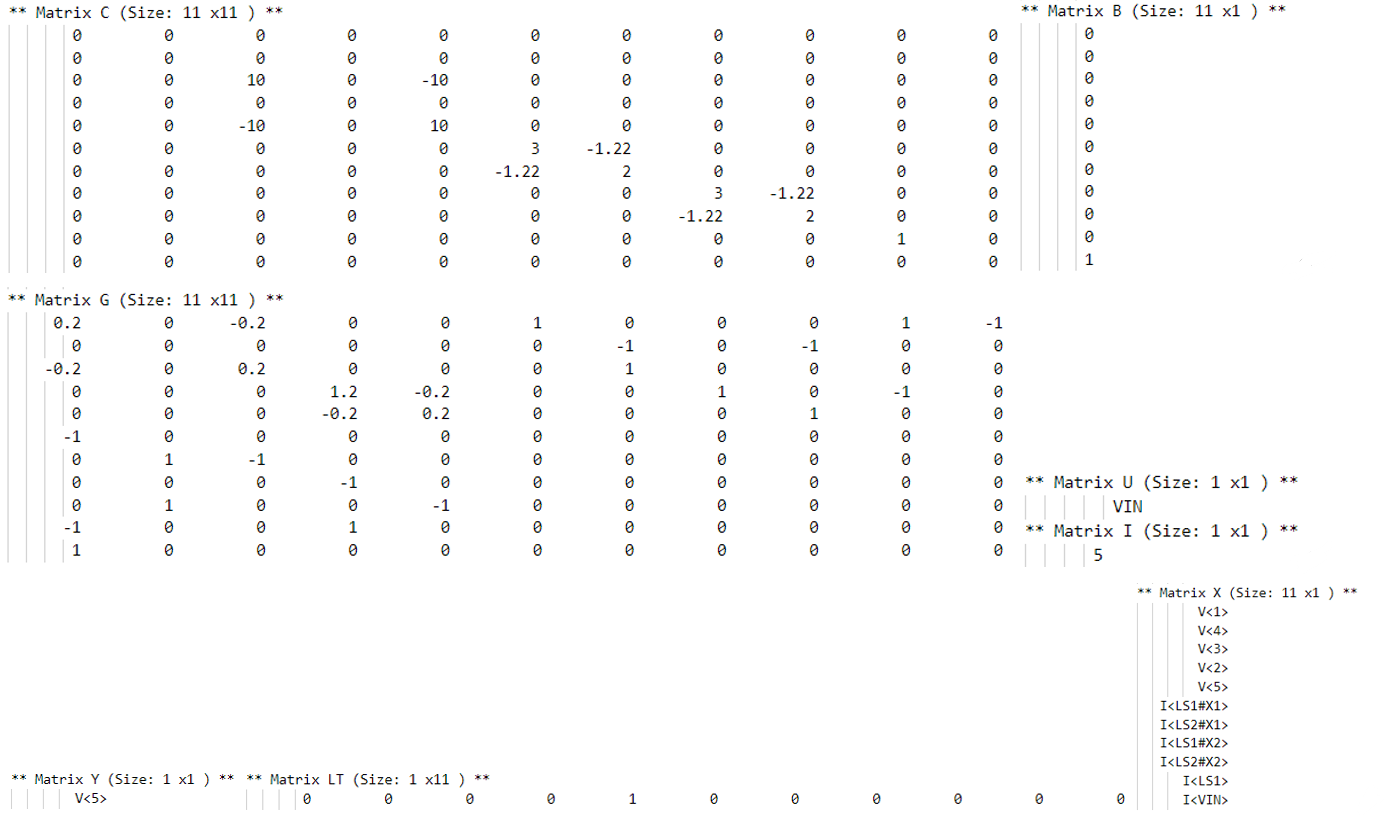
\includegraphics[width=15cm]{figure/Test_full.png}
  \caption{Test\_0全矩阵}
\end{figure}

\begin{figure}[H]
  \centering
  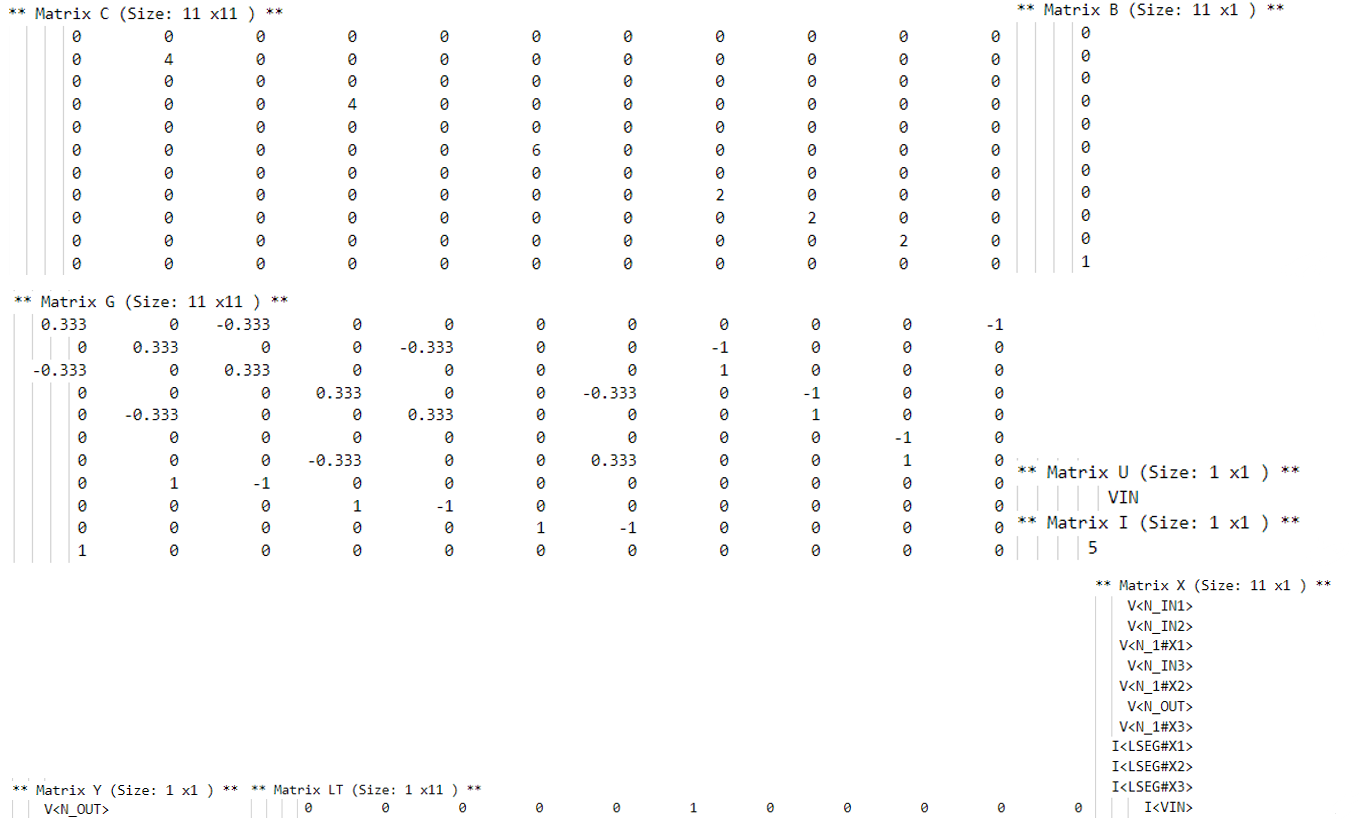
\includegraphics[width=15cm]{figure/RLC_full.png}
  \caption{RLC\_s3全矩阵}
\end{figure}
\qquad 下图为使用编写的read\_matrix函数,在matlab中读取的稀疏矩阵的结果,经过验证稀疏矩阵的数据与完整矩阵的数据一致。\par
\begin{figure}[H]
  \begin{minipage}{0.49\linewidth}
    \centering
    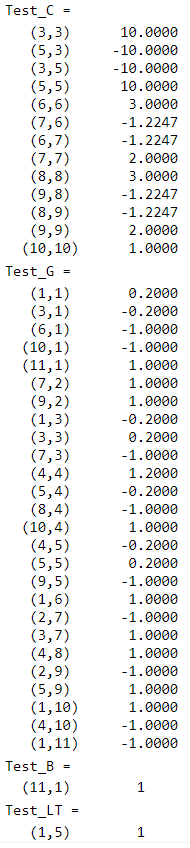
\includegraphics[height=8cm]{figure/Test_sparse.png}
    \caption{Test\_0\ 稀疏矩阵}
  \end{minipage}
  \begin{minipage}{0.49\linewidth}
    \centering
    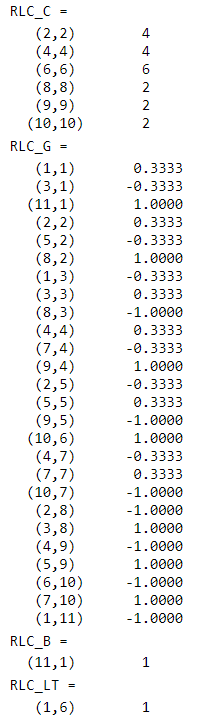
\includegraphics[height=8cm]{figure/RLC_sparse.png}
    \caption{RLC\_s3\ 稀疏矩阵}
  \end{minipage}
\end{figure}

\qquad 下图为RLC例子的分块矩阵输出结果,为了方便对对比同样将矩阵从输出文件中进行截图和拼接(原始数据可参见/output/RLC\_s3\_sub\_matrix.txt),从结果可以看出分块矩阵达到了预期的效果,同时与完整的矩阵结果相同,并且全零矩阵区域在各个例子中都为0。\par
\begin{figure}[H]
  \centering
  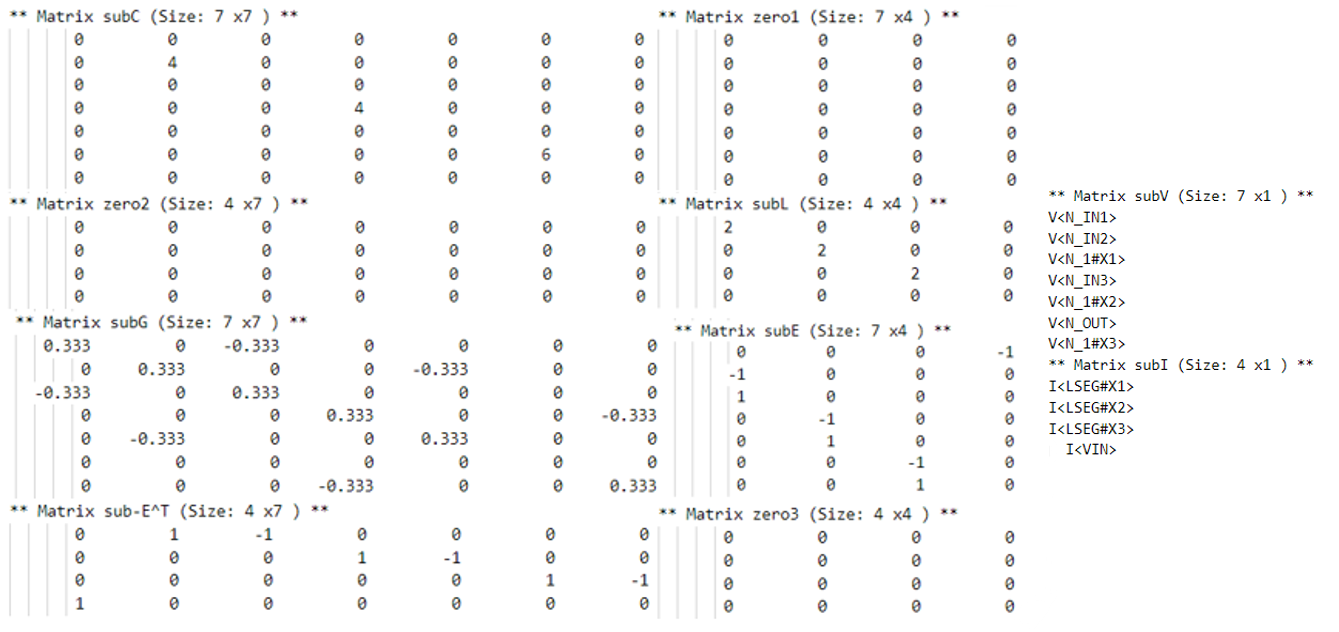
\includegraphics[width=15cm]{figure/RLC_sub.png}
  \caption{Matlab读取二进制文件的矩阵结果}
\end{figure}

\qquad 由于两个大例子Tree和Bus未能展示完整的矩阵,下图展示了matlab读取c++输出二进制文件后的矩阵大小。由于给定的例子中没有受控源,故暂时无法验证其正确性.\par 

\begin{figure}[H]
  \centering
  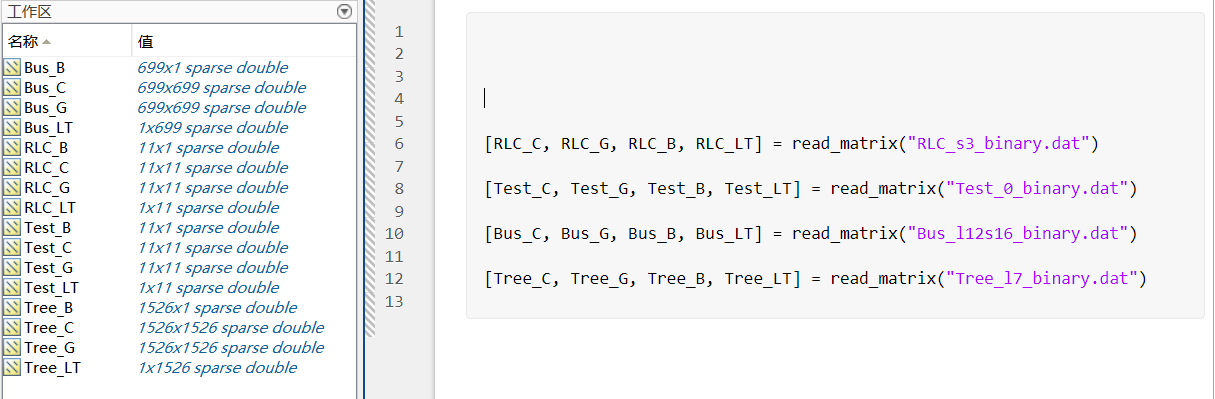
\includegraphics[width=15cm]{figure/all_matrix.png}
  \caption{Matlab读取二进制文件的矩阵结果}
\end{figure}


\section{文件说明}
\qquad 本次项目目录下主要有一下几个子目录:\par
\begin{itemize}
  \item benchmark/:里面为输入的网表文件
  \item output/:输出文件
  \item src/:项目的源代码
  \begin{itemize}
    \item db/ :项目基本的数据类,包括各个元件的hpp文件以及子电路的hpp文件
    \item utils/ :项目用到的一些功能函数,如矩阵hpp文件、解析需要用到的函数以及打log的文件。
    \item CMakeList.txt:cmake配置文件
    \item main.cpp:主函数
    \item stamp.hpp:stamp函数
    \item read\_matrix.mlx:matlab读取二进制文件的函数
    \item test.mlx:matlab测试代码
  \end{itemize}
\end{itemize}

\end{document}